%!TEX root = main-cav.tex

\vspace{-4mm}
\subsection{Summarization of the computations on paths and cycles}\label{sec-sum}
\vspace{-1mm}

Suppose $P=p_0 \xrightarrow{(g_1,\eta_1)} p_1 \dots p_{n-1} \xrightarrow{(g_n,\eta_n)} p_{n}$ is a path of $\Ss$. We assume that the initial values of the control and data variables are represented by a symbolic valuation $\sval$ over $X \cup Y$. 
We use the variables $\vard^{\circled{P}}_1,\vard^{\circled{P}}_2,\dots, \vard^{\circled{P}}_{r^{\circled{P}}}$ to denote the data values introduced while traversing $P$. Notice that according to Proposition~\ref{prop-snt-distinct-value}, one can choose different values for different positions of $P$. Therefore, for each position of $P$, a fresh variable is introduced to represent the data value in that position. Thus we have $r^{\circled{P}}=n$. Here we use the superscript ${\circled{P}}$ to denote the fact that $r^{\circled{P}}$ (resp. $\vard^{\circled{P}}_1$, $\dots$) is associated with the path $P$. 


%for variables $\vard^{\circled{P}}_i,\vard^{\circled{P}}_j$ for $1\leq i< j \leq r^{\circled{P}}$ according to our definition of guards; they will never force the values of $\vard^{\circled{P}}_i$ and $\vard^{\circled{P}}_j$ to be equivalent.


%When $P$ is traversed in a run of $\Ss$ over a data word $w$,  the data value in a position of $w$ may have to be (un)equal to the initial value of some control variable or some other data value in $w$ that have been met before (enforced by the guards and assignments in $P$). Let $\sim$ denote the equivalence relation on $[n]$ induced by $P$ such that $i \sim j$ iff the guards and assignments on $P$ enforce that the data value in the $i$-th position of $w$ must be equal to that in the $j$-th position of $w$. Assuming that there are $r^{\circled{P}}$ ``\emph{fresh}'' equivalence classes of $\sim$, that is, equivalence classes whose values are not enforced to be equivalent to the initial values of control variables. 
%We use the variables $\vard^{\circled{P}}_1,\vard^{\circled{P}}_2,\dots, \vard^{\circled{P}}_{r^{\circled{P}}}$ to denote the data values corresponding to these ``fresh'' equivalence classes, one for each such equivalence class. Note here we use the superscript ${\circled{P}}$ to denote the fact that $r^{\circled{P}}$ (resp. $\vard^{\circled{P}}_1$, $\dots$) is associated with the path $P$.

\hide{ \yfc{hided, we do not have equivalent classes anymore}
\begin{example}
Let $\Ss$ be an SNT where $X=\{x\}$, $Y=\{y\}$, and $P = p_0 \xrightarrow{(g_1,\eta_1)} p_1 \xrightarrow{(g_2,\eta_2)} p_2  \xrightarrow{(g_3,\eta_3)} p_3$ be a path of $\Ss$ such that $(g_1,\eta_1) = (\cur = x, y:= \cur)$, $(g_2,\eta_2)= (\ltrue, (x:=\cur, y:=y+\cur))$, $(g_3,\eta_3)= (\cur=x, y:=y+\cur)$. Then  the guards and assignments enforce that the data value in position $2$ is equal to that in position $3$, that is, $2 \sim 3$. Then the equivalence relation $\sim$ has two equivalence classes, $\{1\}$ and $\{2,3\}$. Moreover, since the data value in position $1$ is equal to the initial value of the control variable $x$, we know that $r^{\circled{P}}=1$, namely, there is only one ``fresh'' equivalence class of $\sim$ (i.e. $\{2,3\}$), and $\vard^{\circled{P}}_1$ is used to denote the data value corresponding to this equivalence class.
\end{example}
}

\begin{proposition}\label{prop-sum-path}
Suppose that $P$ is a path and the initial values of $X \cup Y$ are represented by a symbolic valuation $\initval$. Then the values of $X \cup Y$ after traversing the path $P$ are specified by a symbolic valuation $\sumf^{(P,\initval)}$ satisfying the following conditions.
\begin{itemize}
\item The set of indices of $X$, i.e., $[k]$, is partitioned into $I^{\circled{P}}_{pe}$ and $I^{\circled{P}}_{tr}$, the indices of \emph{persistent} and \emph{transient} control variables, respectively. A control variable is persistent if its value has not been changed while traversing $P$, otherwise, it is transient.
\item For each $x_j\in X$ such that $j\in I^{\circled{P}}_{pe}$, $\sumf^{(P,\initval)}(x_j)=\sval(x_j)$.
%
\item  For each $x_j\in X$ such that $j\in I^{\circled{P}}_{tr}$,
$\sumf^{(P,\initval)}(x_j)=\vard^{\circled{P}}_{\pi^{\circled{P}}(j)}$, where $\pi^{\circled{P}}: I^{\circled{P}}_{tr} \rightarrow [r^{\circled{P}}]$ is a mapping from the index of a transient control variable to the index of the data value assigned to it.
% 
\item For each $y_j \in Y$, 
$
 \sumf^{(P,\initval)}(y_j)  =
 \cste^{\circled{P}}_{j} + 
 \cstl^{\circled{P}}_j \initval(y_j)  + 
  \sum\limits_{j'\in [k]}\csta^{\circled{P}}_{j,j'}\initval(x_{j'}) +
  \sum\limits_{j''\in [r^{\circled{P}}]}\cstb^{\circled{P}}_{j,j''} \vard^{\circled{P}}_{j''}$,
\hide{
\item For each $y_j \in Y$, 
\[
\small
\begin{array}{l}
\smallskip
\sumf^{(P,\initval)}(y_j)  = \\
\hspace{2mm} \cste^{\circled{P}}_{j} + \cstl^{\circled{P}}_j \initval(y_j)  + \csta^{\circled{P}}_{j,1} \initval(x_1) + \dots + \csta^{\circled{P}}_{j,k} \initval(x_k) +  \cstb^{\circled{P}}_{j,1} \vard^{\circled{P}}_1 +\dots + \cstb^{\circled{P}}_{j,r^{\circled{P}}} \vard^{\circled{P}}_{r^{\circled{P}}},
\end{array}
\]} 
where $\cste^{\circled{P}}_j,\cstl^{\circled{P}}_j, \csta^{\circled{P}}_{j,1},\dots,\csta^{\circled{P}}_{j,k}, \cstb^{\circled{P}}_{j,1},\dots,\cstb^{\circled{P}}_{j,r^{\circled{P}}}$ are integer constants such that $\cstl^{\circled{P}}_{j} \in \{0,1\}$ (as a result of the ``independently evolving and copyless'' constraint).  It can happen that $\cstl^{\circled{P}}_j =0$,  which means that $\initval(y_j)$ is irrelevant to $\sumf^{(P,\initval)}(y_j)$. Similarly for $\csta^{\circled{P}}_{j,1}=0$, and so on.
\end{itemize}
\end{proposition}
In Proposition~\ref{prop-sum-path}, the sets $I^{\circled{P}}_{pe}$, $I^{\circled{P}}_{tr}$, the mapping $\pi^{\circled{P}}$, and the constants $\cste^{\circled{P}}_j,\cstl^{\circled{P}}_j, \dots, \cstb^{\circled{P}}_{j,r^{\circled{P}}}$ only depend on $P$ and are independent of $\initval$. In addition, they can be computed in polynomial time from (the transitions in) $P$.
%Due to the uniquely-valued constraint of normalized SNTs, $\pi^{\circled{P}}$ is injective, 
We define $(\pi^{\circled{P}})^{-1}$ as the inverse function of $\pi^{\circled{P}}$, that is, for each $j' \in [r^{\circled{P}}]$, $(\pi^{\circled{P}})^{-1}(j')=\{j \in I^{\circled{P}}_{tr}  \mid \pi^{\circled{P}}(j)= j'\}$. 

As a corollary of Proposition~\ref{prop-sum-path}, the following result demonstrates how to summarize the computations of $\Ss$ on the composition of two paths.

\begin{corollary}\label{cor-comp-two-paths}
Suppose that $P_1$ and $P_2$ are two paths in $\Ss$ such that the last state of $P_1$ is the first state of $P_2$. Moreover, let $\sumf^{(P_1, \initval)}$ (resp. $\sumf^{(P_2, \initval)}$) be the symbolic valuation summarizing the computation of $\Ss$ on $P_1$ (resp. $P_2$). Then the symbolic valuation summarizing the computation of $\Ss$ on $P_1 P_2$ is $\sumf^{(P_2,\ \sumf^{(P_1,\initval)})}$.
\end{corollary}

In order to get a better understanding of the relation between $\sumf^{(P_2,\ \sumf^{(P_1,\initval)})}$ and $(\sumf^{(P_1, \initval)},\sumf^{(P_2, \initval)})$, in the following, for each $y_j \in Y$, we obtain a more explicit form of the expression $\sumf^{(P_2,\ \sumf^{(P_1,\initval)})}(y_j)$, by unfolding therein the expression $\sumf^{(P_1,\initval)}$\medskip.
\resizebox{\hsize}{!}{
	$\begin{array}{rl}
	\medskip
	\sumf^{(P_2,\ \sumf^{(P_1,\initval)})}(y_j) = & 
	\left(\cste^{\circled{P_2}}_{j}+
	\cstl^{\circled{P_2}}_{j} \cste^{\circled{P_1}}_{j}\right)+ \left(\cstl^{\circled{P_2}}_{j} \cstl^{\circled{P_1}}_{j} \right) \initval(y_j)+ \sum \limits_{j' \in I^{\circled{P_1}}_{pe}} 
	\left(\csta^{\circled{P_2}}_{j,j'} +\cstl^{\circled{P_2}}_{j} \csta^{\circled{P_1}}_{j,j'}\right) \initval(x_{j'}) +\\
	\medskip
	& 
	\sum \limits_{j' \in  I^{\circled{P_1}}_{tr}} 
	\left(\cstl^{\circled{P_2}}_{j} \csta^{\circled{P_1}}_{j,j'} \right) \initval(x_{j'}) +
	\sum \limits_{j' \in \rng(\pi^{\circled{P_1}})} \left(\cstl^{\circled{P_2}}_{j} \cstb^{\circled{P_1}}_{j,j'}+\sum \limits_{j'' \in (\pi^{\circled{P_1}})^{-1}(j')} \csta^{\circled{P_2}}_{j,j''} \right) \vard^{\circled{P_1}}_{j'} + 
	 \\
	%
	\smallskip
	& 
	\sum \limits_{j' \in [r^{\circled{P_1}}]\setminus \rng(\pi^{\circled{P_1}})} \left( \cstl^{\circled{P_2}}_{j} \cstb^{\circled{P_1}}_{j,j'} \right) \vard^{\circled{P_1}}_{j'} +
	
	\sum \limits_{j'\in[r^{\circled{P_2}}]} \cstb^{\circled{P_2}}_{j,j'} \vard^{\circled{P_2}}_{j'}.
	\end{array}$
}\medskip\\
In the equation, $j'\in  I^{\circled{P_1}}_{pe}$ implies that $x_{j'}$ remains unchanged when traversing $P_1$, which means the initial value of $x_{j'}$ before traversing $P_2$ is still $\initval(x_{j'})$ and therefore we have the item $ (\csta^{\circled{P_2}}_{j,j'}) \initval(x_{j'})$. When $j' \in \rng(\pi^{\circled{P_1}})$, the initial value of $x_{j''}$ for each $j'' \in (\pi^{\circled{P_1}})^{-1}(j')$ before traversing $P_2$ is $\vard^{\circled{P_1}}_{j'}$ and therefore we have the item $\left(\sum \limits_{j'' \in (\pi^{\circled{P_1}})^{-1}(j')} \csta^{\circled{P_2}}_{j,j''} \right)\ \vard^{\circled{P_1}}_{j'}$.
For all $j'\in [k] = I^{\circled{P_1}}_{pe} \cup I^{\circled{P_1}}_{tr}$, we have the item $(\cstl^{\circled{P_2}}_{j} \csta^{\circled{P_1}}_{j,j'}) \initval(x_{j'})$, i.e. the coefficient of $\initval(x_{j'})$ in $\sumf^{(P_1, \initval)}$ multiplied by $\cstl^{\circled{P_2}}_{j}$. Moreover, for all $j'\in [r^{\circled{P_1}}] = \rng(\pi^{\circled{P_1}}) \cup ([r^{\circled{P_1}}] \setminus \rng(\pi^{\circled{P_1}}))$, we have 
the item $( \cstl^{\circled{P_2}}_{j} \cstb^{\circled{P_1}}_{j,j'}) \vard^{\circled{P_1}}_{j'}$, i.e. the coefficient of $\vard^{\circled{P_1}}_{j'}$ in $\sumf^{(P_1, \initval)}$ multiplied by $\cstl^{\circled{P_2}}_{j}$.

In the following, by utilizing Proposition~\ref{prop-sum-path} and Corollary~\ref{cor-comp-two-paths}, for each path $C^{\ell}$ which is obtained by iterating a cycle $C$ for $\ell$ times, we illustrate how $\sumf^{(C^\ell,\initval)}$ is related to $\sumf^{(C, \initval)}$ and $\ell$. For convenience, we call $\ell$ a \emph{cycle counter variable}.

\begin{proposition}\label{prop-sum-cycle}
Suppose that $C$ is a cycle and $P=C^{\ell}$ such that $\ell \ge 2$. Then the symbolic valuation $\sumf^{(C^\ell,\initval)}$ to summarize the computation of $\Ss$ on $P$ is as follows,\medskip\\
\resizebox{\hsize}{!}{
$\begin{array}{l c l}
\sumf^{(C^\ell,\initval)}(y_j)  & = & 
\left(1 + \cstl^{\circled{C}}_{j} + \dots +(\cstl^{\circled{C}}_{j})^{\ell - 1} \right)\cste^{\circled{C}}_{j} + (\cstl^{\circled{C}}_{j})^\ell \initval(y_j) + \smallskip\\
%
& & \sum \limits_{j' \in I^{\circled{C}}_{pe}} \left(1+\cstl^{\circled{C}}_{j} + \dots +(\cstl^{\circled{C}}_{j})^{\ell - 1} \right) \csta^{\circled{C}}_{j,j'}\initval(x_{j'}) +  \sum \limits_{j' \in I^{\circled{C}}_{tr}}  (\cstl^{\circled{C}}_{j})^{\ell - 1} \csta^{\circled{C}}_{j,j'} \initval(x_{j'}) +  \\
%
& & \sum \limits_{j' \in \rng(\pi^{\circled{C}})} \sum \limits_{s\in[\ell -1]}
\left(\cstl^{\circled{C}}_{j}\cstb^{\circled{C}}_{j,j'}+ \sum \limits_{j'' \in (\pi^{\circled{C}})^{-1}(j')} \csta^{\circled{C}}_{j, j''}  \right)
(\cstl^{\circled{C}}_{j})^{\ell-s-1}
\vard^{\circled{C , s}}_{j'} +\\
%
& & \sum \limits_{j' \in [r^{\circled{C}}] \setminus \rng(\pi^{\circled{C}})}\sum \limits_{s\in[\ell -1]} \left((\cstl^{\circled{C}}_{j})^{\ell - s} \cstb^{\circled{C}}_{j,j'} \right) \vard^{\circled{C , s}}_{j'} + 
\sum \limits_{j' \in [r^{\circled{C}}] }  
 \cstb^{\circled{C}}_{j, j'} \vard^{\circled{C , \ell}}_{j'},
\end{array} 
$}\medskip\\
where the variables $\vard^{\circled{C , s}}_{1},\dots, \vard^{\circled{C ,s}}_{r^{\circled{C}}}$ for $s\in [\ell]$
 represent the data values introduced when traversing $C$ for the $s$-th time.
\end{proposition}

From Proposition~\ref{prop-sum-cycle} and the fact that $\cstl_{j} \in \{0, 1\}$, we have the following observation.
\begin{itemize}
\item If $\cstl^{\circled{C}}_{j}=0$, then\medskip\\
\resizebox{0.9\hsize}{!}{$
\sumf^{(C^\ell,\initval)}(y_j)   =  \cste^{\circled{C}}_{j} +  \sum \limits_{j' \in I^{\circled{C}}_{pe}} \csta^{\circled{C}}_{j,j'} \initval(x_{j'}) +
\sum \limits_{j'  \in \rng(\pi^{\circled{C}})} \left(\sum \limits_{j'' \in (\pi^{\circled{C}})^{-1}(j')} \csta^{\circled{C}}_{j, j''} \right) \vard^{\circled{C , \ell  -  1}}_{j'} + \sum \limits_{j' \in [r^{\circled{C}}] }  
\cstb^{\circled{C}}_{j, j'} \vard^{\circled{C , \ell}}_{j'}.$}


\item If $\cstl^{\circled{C}}_{j}=1$, then\medskip\\
\resizebox{0.95\hsize}{!}{$
\begin{array}{l }
\sumf^{(C^\ell,\initval)}(y_j)  =    \ell \cste^{\circled{C}}_{j}  + \initval(y_j) +   \sum  \limits_{j' \in I^{\circled{C}}_{pe}} \ell \csta^{\circled{C}}_{j,j'}  \initval(x_{j'}) + 
\sum \limits_{j' \in I^{\circled{C}}_{tr}} \csta^{\circled{C}}_{j,j'} \initval(x_{j'}) +  \smallskip\\
\sum \limits_{j' \in \rng(\pi^{\circled{C}})} \sum \limits_{s\in[\ell -1]}
\left(\cstb^{\circled{C}}_{j,j'} + \sum \limits_{j'' \in (\pi^{\circled{C}})^{-1}(j')} \csta^{\circled{C}}_{j, j''}   \right) \vard^{\circled{C , s}}_{j'} + \sum \limits_{j' \in [r^{\circled{C}}]  \setminus \rng(\pi^{\circled{C}}) }\sum \limits_{s\in[\ell -1]} 
\cstb^{\circled{C}}_{j,j'} \vard^{\circled{C , s}}_{j'} + \sum \limits_{j' \in [r^{\circled{C}}] }  
\cstb^{\circled{C}}_{j, j'} \vard^{\circled{C , \ell}}_{j'}.
\end{array}
$}
%



\hide{
\item If $\alpha^{\circled{C}}_{j,1}=-1$ and $\ell$ is even, then
\[
\begin{array}{l c l}
\chi^{\circled{C}}_{\ell}(y_j)  & = &  o_j + \sum \limits_{j'\le k, \pi_C(j') \neq j'} (-\beta^{\circled{C}}_{j,j'}) d^{(0)}_{j'} +  \\
%
& & \sum \limits_{j' \le r_C ,  j'+k \in \rng(\pi_C)} ( \beta^{\circled{C}}_{j, \pi_C^{-1}(j'+k)} - \gamma^{\circled{C}}_{j,j'}) d^{\circled{C , 1}}_{j'} + \\
%
& & \sum \limits_{j' \le r_C ,   j'+k \not \in \rng(\pi_C)} (-\gamma^{\circled{C}}_{j,j'}) d^{\circled{C , 1}}_{j'} + \dots + \\
%
& & \sum \limits_{j' \le r_C ,  j'+k \in \rng(\pi_C)} (\beta^{\circled{C}}_{j, \pi_C^{-1}(j'+k)}-\gamma^{\circled{C}}_{j,j'}) d^{\circled{C , \ell  -  1}}_{j'} + \\
%
& & \sum \limits_{j' \le r_C ,   j'+k \not \in \rng(\pi_C)} (-\gamma^{\circled{C}}_{j,j'}) d^{\circled{C , \ell  -  1}}_{j'} + \gamma^{\circled{C}}_{j, 1} d^{\circled{C , \ell}}_{1} + \dots + \gamma^{\circled{C}}_{j,r_C} d^{\circled{C , \ell}}_{r_C}.
\end{array} 
\]
\item If $\alpha_{j,1}=-1$ and $\ell$ is odd, then
\[
\begin{array}{l c l}
\smallskip
\chi^{\circled{C}}_{\ell}(y_j)  & = &  \alpha^{\circled{C}}_{j,0} - o_j + \sum \limits_{j' \le k, \pi_C(j')=j'} \beta^{\circled{C}}_{j,j'} d^{(0)}_{j'} +  \sum \limits_{j'\le k, \pi_C(j') \neq j'}  \beta^{\circled{C}}_{j,j'} d^{(0)}_{j'} +  \\
%
& & \sum \limits_{j' \le r_C ,  j'+k \in \rng(\pi_C)} ( -\beta^{\circled{C}}_{j, \pi_C^{-1}(j'+k)} +\gamma^{\circled{C}}_{j,j'}) d^{\circled{C , 1}}_{j'} + \\
%
& & \sum \limits_{j' \le r_C ,   j'+k \not \in \rng(\pi_C)} \gamma^{\circled{C}}_{j,j'} d^{\circled{C , 1}}_{j'} + \dots + \\
%
& & \sum \limits_{j' \le r_C ,  j'+k \in \rng(\pi_C)} (\beta^{\circled{C}}_{j, \pi_C^{-1}(j'+k)}-\gamma^{\circled{C}}_{j,j'}) d^{\circled{C , \ell  -  1}}_{j'} + \\
%
& & \sum \limits_{j' \le r_C ,   j'+k \not \in \rng(\pi_C)} (-\gamma^{\circled{C}}_{j,j'}) d^{\circled{C , \ell  -  1}}_{j'} + \gamma^{\circled{C}}_{j, 1} d^{\circled{C , \ell}}_{1} + \dots + \gamma^{\circled{C}}_{j,r_C} d^{\circled{C , \ell}}_{r_C}.
\end{array} 
\]
}
\end{itemize}

%
%From the analysis above, we observe that in $\chi^{\circled{C}}_\ell(y_j)$, 
%\begin{itemize}
%\item the constant coefficient is either $\alpha^{\circled{C}}_{j,0}$, or $\alpha^{\circled{C}}_{j,0} \ell$, 
%
%\item the coefficient of $o_j$ is $0$, or $1$, 
%
%\item for each data value $d^{(0)}_{j'}$, the coefficient of $d^{(0)}_{j'}$ is either $\beta^{\circled{C}}_{j,j'}$, or $0$, or $\beta^{\circled{C}}_{j,j'} \ell$,
%
%\item for each data value $d^{(C , i)}_{j'}$ with $i \ge 1$, the coefficient of $d^{(C , i)}_{j'}$ is either $0$, or $\beta^{\circled{C}}_{j, \pi_C^{-1}(j'+k)}$, or $\beta^{\circled{C}}_{j, \pi_C^{-1}(j'+k)}+\gamma^{\circled{C}}_{j,j'}$, or $\gamma^{\circled{C}}_{j,j'}$.
%\end{itemize}

\begin{example}\label{exmp-sum}
Let $\Ss'_{\sf max}$ be the SNT illustrated in Fig.~\ref{fig-dec-proc-snt-exmp}, which is obtained from $\Ss_{\sf max}$ by replacing  the control variable $\sf max$ with  $x_1$ and introducing the data variables $y_1,y_2, y_3$. Consider the cycle $C_1$ in $\Ss'_{\sf max}$. Then $O(q_2)= a_0 + a_1 x_1 + b_1 y_1 + b_2 y_2 + b_3 y_3 = y_1 - 2y_2 + y_3$, $I^{\circled{C_1}}_{pe} = \{1\}$, $I^{\circled{C_1}}_{tr} = \emptyset$, $\cstl^{\circled{C_1}}_1 = \cstl^{\circled{C_1}}_2 = 1$, $\cstl^{\circled{C_1}}_3 = 0$, moreover, suppose $\ell \ge 2$, let $ \vard^{\circled{C_1, 1}}_1, \dots, \vard^{\circled{C_1, \ell}}_1$ represent the data values introduced when traversing the path $C^\ell_1$, then
\[
\begin{array}{l c l}
\sumf^{(C^\ell_1, \initval)}(y_1) &= & \initval(y_1) + (4 \ell) \initval(x_1) +\ \ \vard^{\circled{C_1, 1}}_1 + \dots +\ \ \vard^{\circled{C_1, \ell}}_1,\\
%
\sumf^{(C^\ell_1, \initval)}(y_2) &=& \initval(y_2) + (2 \ell) \initval(x_1) + 2 \vard^{\circled{C_1, 1}}_1 + \dots + 2 \vard^{\circled{C_1, \ell}}_1,\\
%
\sumf^{(C^\ell_1, \initval)}(y_3) &=& \hspace{5.5cm} 3 \vard^{\circled{C_1, \ell}}_1,
\end{array}
\] 
on the other hand, $I^{\circled{C_2}}_{pe} = \emptyset$, $I^{\circled{C_2}}_{tr} = \{1\}$, $\cstl^{\circled{C_2}}_1 = \cstl^{\circled{C_2}}_2 = \cstl^{\circled{C_2}}_3  = 1$, let $ \vard^{\circled{C_2, 1}}_1, \dots, \vard^{\circled{C_2, \ell}}_1$ represent the data values introduced when traversing the path $C^\ell_2$, then 
\[
\begin{array}{l c l}
\sumf^{(C^\ell_2, \initval)}(y_1) &= & \initval(y_1) +\ \  \initval(x_1) +4 \vard^{\circled{C_2, 1}}_1 + \dots +4 \vard^{\circled{C_2, \ell-1}}_1 + 3 \vard^{\circled{C_2, \ell}}_1,\\
%
\sumf^{(C^\ell_2, \initval)}(y_2) &=& \initval(y_2) + 3 \initval(x_1) + 5 \vard^{\circled{C_2, 1}}_1 + \dots + 5 \vard^{\circled{C_2, \ell-1}}_1 + 2 \vard^{\circled{C_2, \ell}}_1,\\
%
\sumf^{(C^\ell_2, \initval)}(y_3) &=& \initval(y_3) + 5 \initval(x_1) + 6 \vard^{\circled{C_2, 1}}_1 + \dots + 6 \vard^{\circled{C_2, \ell-1}}_1 + \ \ \vard^{\circled{C_2, \ell}}_1.
\end{array}
\] 
\begin{figure}[htbp]
\begin{center}
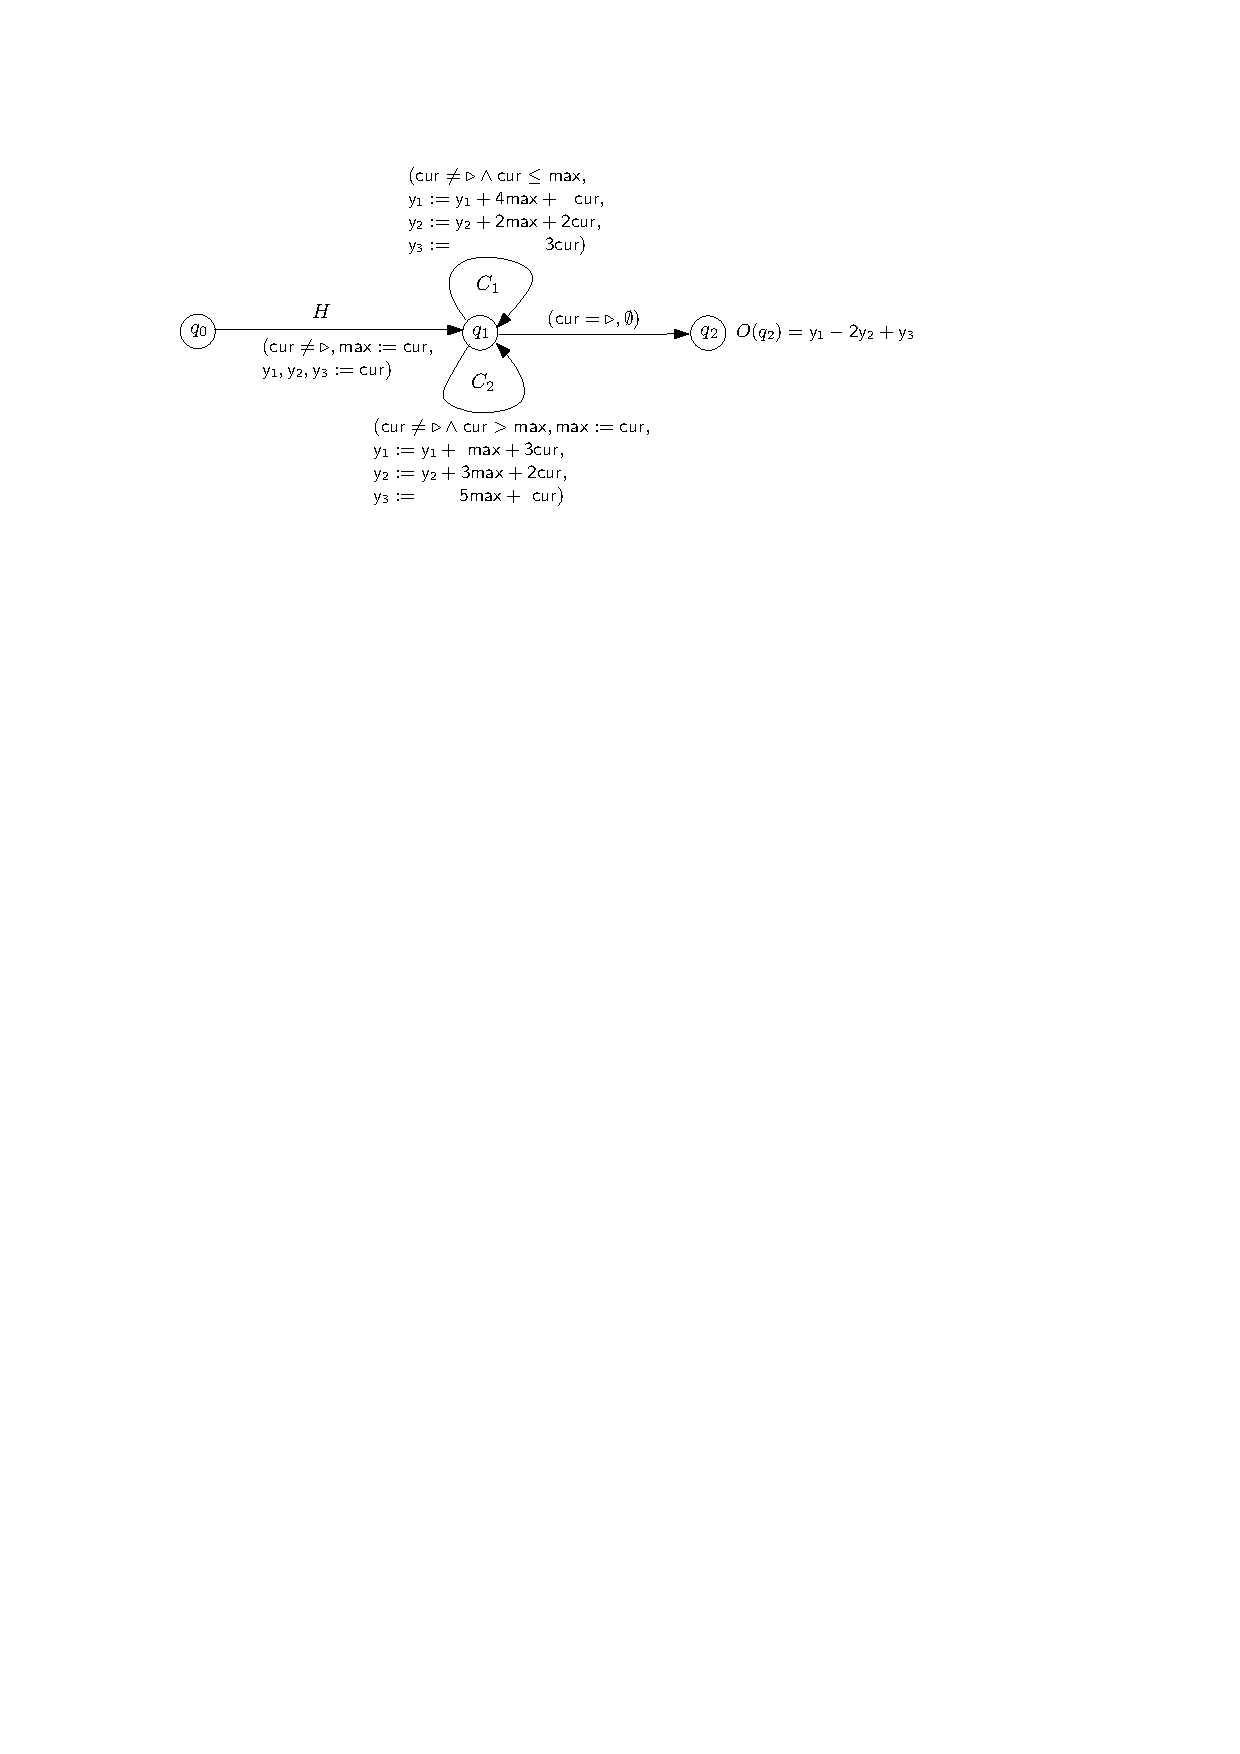
\includegraphics[scale=0.9]{dec-proc-snt-exmp.pdf}
\caption{The SNT $\Ss'_{\max}$: Extending $\Ss_{\max}$ with data variables}\label{fig-dec-proc-snt-exmp}
\end{center}
\end{figure}
%
\end{example}
